\documentclass{standalone}
\usepackage{tikz}
\usetikzlibrary{arrows.meta, positioning, shapes, calc}

\begin{document}
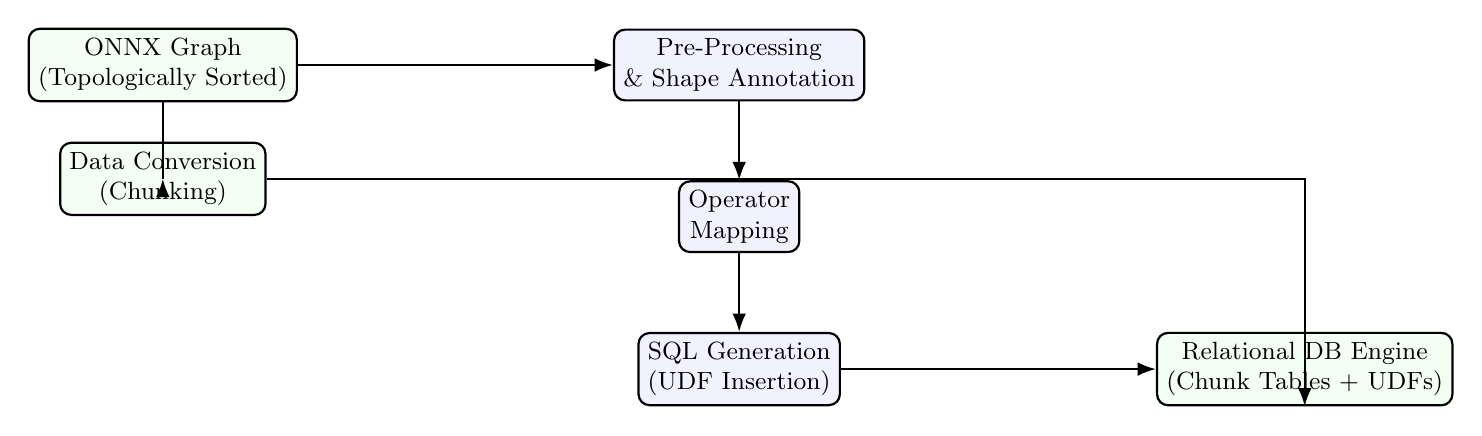
\begin{tikzpicture}[
    font=\sffamily,
    >=LaTeX,
    node distance=15mm and 25mm,
    line/.style={draw, thick, ->},
    block/.style={rectangle, draw, rounded corners, align=center, minimum height=1.2em,
                  minimum width=2.5em, font=\small, thick, fill=blue!5},
    io/.style={rectangle, draw, rounded corners, align=center, minimum height=1.2em,
               minimum width=2.5em, font=\small, thick, fill=green!5}
]

% NODES
\node[io] (onnx) {ONNX Graph \\ (Topologically Sorted)};
\node[block, right=of onnx, xshift=15mm] (pre) {Pre-Processing \\ \& Shape Annotation};
\node[block, below=of pre, yshift=5mm] (map) {Operator \\ Mapping};
\node[block, below=of map, yshift=5mm] (sqlgen) {SQL Generation \\ (UDF Insertion)};

\node[io, right=of sqlgen, xshift=15mm] (db) {Relational DB Engine \\ (Chunk Tables + UDFs)};

\node[io, below=of onnx, yshift=10mm] (data) {Data Conversion \\ (Chunking)};

% DRAW LINES
\draw[line] (onnx) -- (pre);
\draw[line] (pre) -- (map);
\draw[line] (map) -- (sqlgen);
\draw[line] (sqlgen) -- (db);

\draw[line] (onnx) |- node[left, near start] {} (data);

% OPTIONAL: Show that data conversion feeds into the DB as chunked tables
\draw[line] (data.east) -| node[near start, above] {} (db.south);

% LEGEND (Optional)
%\node[align=left, font=\small] at ($(db.east)+(2.6,0)$)
%{%
%  \textbf{Legend:}\\
%  \textcolor{blue!70!black}{\rule{1em}{0.6em}} = Processing Stage \\
%  \textcolor{green!70!black}{\rule{1em}{0.6em}} = Input/Output
%};

\end{tikzpicture}
\end{document}
